% !TeX root = bagrut-all.tex

\selectlanguage{hebrew}

\chapter{מעגל היחידה}\label{a.unit-circle}

\section*{רביעים של מעגל היחידה}

מעגל שהרדיוס שלו 
$1$
נקרא
\textbf{מעגל היחידה}.

\vspace{-2ex}

\begin{center}
\selectlanguage{english}
% The unit circle
\begin{tikzpicture}[scale=1.8]
\coordinate (origin) at (0,0);
% Draw circle
\draw[name path=circle] (origin) node [above left] {$(0,0)$} circle [radius=1];
% Draw axes
\draw[name path=x] (-1,0) node [left] {$(-1,0)$} -- (1,0) node [right] {$(1,0)$};
\draw (0,-1) node [below] {$(0,-1)$} -- (0,1) node [above] {$(0,1)$};
% Draw ray
\draw[rotate=30,name path=ray] (origin) node [above right,xshift=8mm] {$\theta$} -- node [above] {$1$} (1,0);
% Get intersection of circle and ray
\path [name intersections={of=circle and ray, by=on-circle}];
% Draw altitude from intersection to x-axis
\draw[name path=altitude] (on-circle) node[above right] {$(\cos\theta,\sin\theta)$} -- node [right,xshift=4mm] {$\sin \theta$} (on-circle |- origin);
\draw[->] (1.1,.25) -- +(-6pt,0);
% Get intersection of altitude and x-axis
\path [name intersections={of=altitude and x, by=on-x}] (origin) -- node [below] {$\cos \theta$} (on-x);
% Square for right angle at intersection
\draw (on-x) rectangle +(-2pt,2pt);
% Dot at origin
\fill (origin) circle [radius=1pt];
\end{tikzpicture}
\end{center}

\vspace{-3ex}

הצירים של מעגל היחידה מחלקים אותו באופן טבעי לארבעה
\textbf{רביעים}.
זוויות נמדדות 
\textbf{במעלות}
בין
$0^\circ$
ל-%
$\pm 360^\circ$,
כאשר הערכים חיוביים אם מודדים נגד כיוון השעון, ושליליים עם כיוון השוען.

יחידה אחרת לזווית היא ה-%
\textbf{רדיאן}.
רדיאן אחד הוא הזווית הכולאת קשת שאורכו שווה לרדיוס. במעגל היחידה הרדיוס הוא
$1$
ולכן אורך ההיקף הוא
$2\pi$.
רדיאן אחד שווה בערך
$57.3$	
מעלות.
\begin{center}
\selectlanguage{english}
% The unit circle with main axes
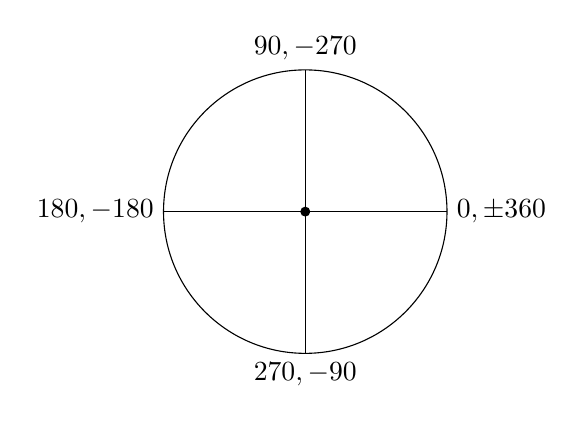
\begin{tikzpicture}[scale=1.8]
\coordinate (origin) at (0,0);
% Draw circle
\draw (origin) circle [radius=1];
% Draw axes
\draw (-1,0) node [left] {$180,-180$} -- (1,0) node [right] {$0,\pm 360$};
\draw (0,-1) node [below] {$270,-90$} -- (0,1) node [above] {$90,-270$};
% Dot at origin
\fill (origin) circle [radius=1pt];
\end{tikzpicture}
\hspace{3em}
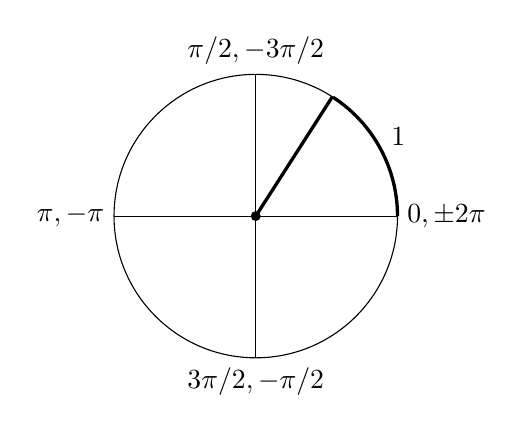
\begin{tikzpicture}[scale=1.8]
\coordinate (origin) at (0,0);
% Draw circle
\draw (origin) circle [radius=1];
% Draw axes
\draw (-1,0) node [left] {$\pi,-\pi$} -- (1,0) node [right] {$0,\pm 2\pi$};
\draw (0,-1) node [below] {$3\pi/2,-\pi/2$} -- (0,1) node [above] {$\pi/2,-3\pi/2$};
% Draw one radian
\draw[very thick] (origin) -- (57.3:1);
\draw[very thick]  (1,0) arc(0:57:1);
\node at (29:1.15) {$1$};
% Dot at origin
\fill (origin) circle [radius=1pt];
\end{tikzpicture}
\end{center}

מהחיתוכים של הצירים עם מעגל היחידה נקבל את ערכי הסינוס והקוסינוס של הזוויות:
\begin{displaymath}
\erh{6pt}
\begin{array}{|c|c|c|c|}
\hline
\textrm{\R{זווית}} & \textrm{\R{זווית}} & \sin & \cos\\
\textrm{(\R{מעלות})} & \textrm{(\R{רדיאנים})} & & \\\hline
0 & 0 & 0 & 1\\\hline
90,-270 & \pi/2, -3\pi/2 & 1 & 0\\\hline
180, -180 & \pi,-\pi & 0 & -1\\\hline
270,-90 & 3\pi/2,-\pi/2 & -1 & 0\\
\hline
\end{array}
\end{displaymath}

\np

%%%%%%%%%%%%%%%%%%%%%%%%%%%%%%%%%%%%%%%%%%%%%%%%%%%%%%%%%%%%%%%


\section*{%
חלוקת מעגל היחידה ל-%
$8$
קטעים
}

נחלק כל רביע בחצי ונקבל
$8$
קטעים. הזווית של כל קטע הוא
$45^\circ$
או
$\pi/4$
רדיאנים:
\begin{center}
\selectlanguage{english}
% The unit circle divided into 45 degree segments
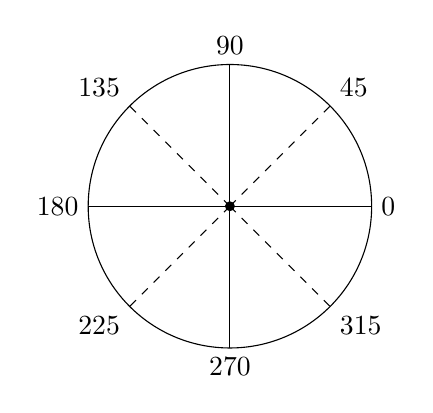
\begin{tikzpicture}[scale=1.8]
\coordinate (origin) at (0,0);
% Draw circle
\draw (origin) circle [radius=1];
% Draw axes
\draw (-1,0) node [left] {$180$} -- (1,0) node [right] {$0$};
\draw (0,-1) node [below] {$270$} -- (0,1) node [above] {$90$};
% Draw other angles
\draw[dashed] (origin) -- +(45:1) node[above right] {$45$};
\draw[dashed] (origin) -- +(135:1) node[above left] {$135$};
\draw[dashed] (origin) -- +(225:1) node[below left] {$225$};
\draw[dashed] (origin) -- +(315:1) node[below right] {$315$};
% Dot at origin
\fill (origin) circle [radius=1pt];
\end{tikzpicture}
\hspace{5em}
% The unit circle with radians divided into pi/4 segments
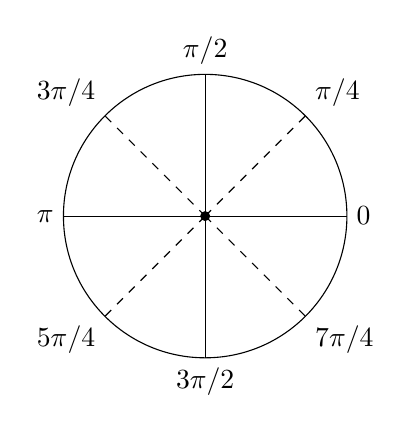
\begin{tikzpicture}[scale=1.8]
\coordinate (origin) at (0,0);
% Draw circle
\draw (origin) circle [radius=1];
% Draw axes
\draw (-1,0) node [left] {$\pi$} -- (1,0) node [right] {$0$};
\draw (0,-1) node [below] {$3\pi/2$} -- (0,1) node [above] {$\pi/2$};
% Draw other angles
\draw[dashed] (origin) -- +(45:1) node[above right] {$\pi/4$};
\draw[dashed] (origin) -- +(135:1) node[above left] {$3\pi/4$};
\draw[dashed] (origin) -- +(225:1) node[below left] {$5\pi/4$};
\draw[dashed] (origin) -- +(315:1) node[below right] {$7\pi/4$};
% Dot at origin
\fill (origin) circle [radius=1pt];
\end{tikzpicture}
\end{center}


במשולש 
$\triangle ABC$
אם הזווית
$\angle BAC$
היא
$45^\circ$,
הזווית הנגדית
$\angle ABC$
גם היא
$45^\circ$
כדי שסכום הזוויות במשולש יהיה
$180^\circ$.
המשולש שווי-שוקיים כך שערכי הסינוס והקוסינוס שווים. 
\begin{center}
\selectlanguage{english}
% Right triangle with 45 degree angles
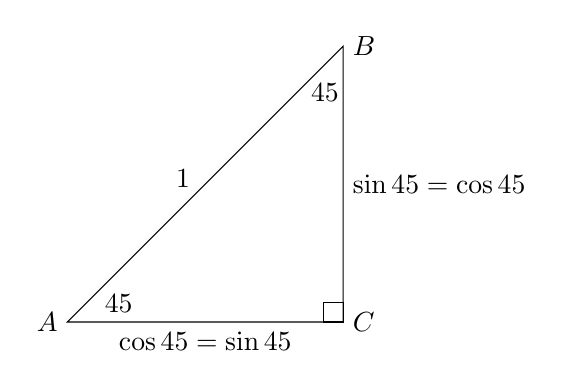
\begin{tikzpicture}[scale=3.5]
% Coordinates
\coordinate (origin) at (0,0);
\coordinate (lower-right) at (1,0);
\coordinate (upper-right) at (1,1);
% Draw triangle
\draw (origin) node[left] {$A$} node[above right,xshift=10pt] {$45$} -- node[below] {$\cos 45=\sin 45$} (lower-right) node[right] {$C$} -- node[right] {$\sin 45=\cos 45$} (upper-right) node[right] {$B$} node[below left,xshift=2pt,yshift=-10pt] {$45$} -- node[left,xshift=-2pt,yshift=2pt] {$1$} cycle;
% Square for right angle
\draw (lower-right) rectangle +(-2pt,2pt);
\end{tikzpicture}
\end{center}
ממשפט פיתגורס:
\erh{14pt}
\begin{equationarray*}{rcl}
\sin^2 45 + \cos^2 45 &=& 1\\
2\sin^2 45 &=& 1\\
\sin 45 = \cos 45&=& \frac{1}{\sqrt{2}} = \frac{1}{\sqrt{2}}\cdot \frac{2}{2} =\frac{\sqrt{2}}{2}\,.
\end{equationarray*}

%%%%%%%%%%%%%%%%%%%%%%%%%%%%%%%%%%%%%%%%%%%%%%%%%%%%%%%%%%%%%%%

\section*{סינוס וקוסינוס של זוויות הגדולות מ-%
$90^\circ$}

עכשיו שאנו יודעים את ערכי הסינוס והקוסינוס של
$45^\circ$,
נוכל לשאול על הזוויות הסימטריות
$135^\circ=180^\circ\!-\!45^\circ$, $225^\circ=180^\circ\!+\!45^\circ$, $315^\circ=-45^\circ$.
בתרשימים שלהלן סימנו את הזוויות הסימטריות עבור זווית שרירותית
$\theta$
ברביע הראשון. ערכי ה-%
$x,y$
שווים פרט לסימנים.

\np

ברביע השני:
\begin{center}
\selectlanguage{english}
% Functions of 180-\theta
\begin{tikzpicture}[scale=2]
\coordinate (origin) at (0,0);
% Draw circle
\draw[name path=circle] (origin) circle [radius=1];
% Draw axes
\draw (-1,0) -- (1,0);
\draw (0,-1) -- (0,1);
% Draw first ray
\path[name path=ray1] (origin) -- +(40:1.1);
\path[name intersections={of=circle and ray1,by=on-circle1}];
\draw (origin) node[above right,xshift=14pt,yshift=-1pt] {$\theta$} -- (on-circle1) node[above right,xshift=-4pt] {$(\cos \theta, \sin \theta)$};
% Draw altitude and square for right angle
\draw[dashed] (on-circle1) -- (on-circle1 |- origin);
\draw (on-circle1 |- origin) rectangle +(-2pt,2pt);
% Draw second ray
\path[name path=ray2] (origin) -- +(140:1.1);
\path[name intersections={of=circle and ray2,by=on-circle2}];
\draw (origin) -- (on-circle2) node[above left,xshift=4pt] {$(-\cos \theta, \sin \theta)$};
% Draw altitude and square for right angle
\draw[dashed] (on-circle2) -- (on-circle2 |- origin);
\draw (on-circle2 |- origin) rectangle +(2pt,2pt);
% Draw the arc for 180-\theta
\draw (12pt,0) arc(0:140:12pt);
\node at (8pt,18pt) {$180-\theta$};
\draw[->] (6pt,16pt) -- +(0,-4pt);
\end{tikzpicture}
\end{center}

\vspace{-2ex}

\[
\cos 135=-\cos 45= \displaystyle -\frac{\sqrt{2}}{2},\quad\quad \sin 135=\sin 45= \displaystyle \frac{\sqrt{2}}{2}\,.
\]

\vspace{-4ex}

ברביע השלישי והרביעי:
\begin{center}
\selectlanguage{english}
% Functions of 180+\theta
\begin{tikzpicture}[scale=1.8]
\coordinate (origin) at (0,0);
% Draw circle
\draw[name path=circle] (origin) circle [radius=1];
% Draw axes
\draw (-1,0) -- (1,0);
\draw (0,-1) -- (0,1);
% Draw first ray
\path[name path=ray1] (origin) -- +(40:1.1);
\path[name intersections={of=circle and ray1,by=on-circle1}];
\draw (origin) node[above right,xshift=14pt,yshift=-1pt] {$\theta$} -- (on-circle1) node[above right,xshift=-4pt] {\shortstack{$(\cos \theta,$\\$\sin \theta)$}};
% Draw altitude and square for right angle
\draw[dashed] (on-circle1) -- (on-circle1 |- origin);
\draw (on-circle1 |- origin) rectangle +(-2pt,2pt);
% Draw second ray
\path[name path=ray2] (origin) -- +(-140:1.1);
\path[name intersections={of=circle and ray2,by=on-circle2}];
\draw (origin) -- (on-circle2) node[below left,xshift=4pt] {\shortstack{$(-\cos \theta,$\\$-\sin \theta)$}};
% Draw altitude and square for right angle
\draw[dashed] (on-circle2) -- (on-circle2 |- origin);
\draw (on-circle2 |- origin) rectangle +(2pt,-2pt);
% Draw the arc for 180+\theta
\draw (12pt,0) arc(0:220:12pt);
\node at (8pt,18pt) {$180+\theta$};
\draw[->] (6pt,16pt) -- +(0,-4pt);
\end{tikzpicture}
\hspace{3em}
% Functions of -\theta
\begin{tikzpicture}[scale=1.8,baseline=-66pt]
\coordinate (origin) at (0,0);
% Draw circle
\draw[name path=circle] (origin) circle [radius=1];
% Draw axes
\draw (-1,0) -- (1,0);
\draw (0,-1) -- (0,1);
% Draw first ray
\path[name path=ray1] (origin) -- +(40:1.1);
\path[name intersections={of=circle and ray1,by=on-circle1}];
\draw (origin) node[above right,xshift=12pt] {$\theta$} -- (on-circle1) node[right,xshift=4pt] {\shortstack{$(\cos \theta,$\\$\sin \theta)$}};
% Draw altitude and square for right angle
\draw[dashed] (on-circle1) -- (on-circle1 |- origin);
\draw (on-circle1 |- origin) rectangle +(-2pt,2pt);
% Draw second ray
\path[name path=ray2] (origin) -- +(-40:1.1);
\path[name intersections={of=circle and ray2,by=on-circle2}];
\draw (origin) node[below right,xshift=13pt] {$-\theta$} -- (on-circle2) node[right,xshift=4pt] {\shortstack{$(\cos \theta,$\\$-\sin \theta)$}};
% Draw altitude and square for right angle
\draw[dashed] (on-circle2) -- (on-circle2 |- origin);
\draw (on-circle2 |- origin) rectangle +(-2pt,-2pt);
\end{tikzpicture}
\end{center}
\vspace{-3ex}

\[
\begin{array}{ll}
\cos 225 = -\cos 45= \displaystyle -\frac{\sqrt{2}}{2},\quad\quad &\sin 225 = -\sin 45= \displaystyle -\frac{\sqrt{2}}{2}\\
\cos 315=\cos 45= \displaystyle \frac{\sqrt{2}}{2},\quad\quad &\sin 315=-\sin 45= \displaystyle -\frac{\sqrt{2}}{2}\,.
\end{array}
\]
נסכם את הערכים בטבלה:
\begin{displaymath}
\renewcommand{\arraystretch}{.7}
\begin{array}{|c|c|c|c|}
\hline
\textrm{\R{זווית}} & \textrm{\R{זווית}} & \sin & \cos\\
\textrm{(\R{מעלות})} & \textrm{(\R{רדיאנים})} & & \\\hline
\theta& \theta&  \sin\theta &  \cos\theta \\\hline
180\!-\!\theta& \pi\!-\!\theta&  \sin\theta &  -\cos\theta\\\hline
180+\theta& \pi+\theta&  -\sin\theta &  -\cos\theta\\\hline
-\theta& \theta&  -\sin\theta &  \cos\theta\\
\hline
\end{array}
\end{displaymath}

\np
ועבור
$45^\circ$:
\begin{displaymath}
\renewcommand{\arraystretch}{.8}
\begin{array}{|c|c|c|c|}
\hline
\textrm{\R{זווית}} & \textrm{\R{זווית}} & \sin & \cos\\
\textrm{(\R{מעלות})} & \textrm{(\R{רדיאנים})} & & \\\hline
45& \pi/4&  \sqrt{2}/2 &  \sqrt{2}/2 \\\hline
135& 3\pi/4&  \sqrt{2}/2 &  -\sqrt{2}/2\\\hline
225& 5\pi/4&  -\sqrt{2}/2 &  -\sqrt{2}/2\\\hline
315& 7\pi/4&  -\sqrt{2}/2 &  \sqrt{2}/2\\
\hline
\end{array}
\end{displaymath}

%%%%%%%%%%%%%%%%%%%%%%%%%%%%%%%%%%%%%%%%%%%%%%%%%%%%%%%%%%%%%%%

\section*{הסינוס והקוסינוס של
$30^\circ$
ו
$60^\circ$}

את מעגל היחידה ניתן לחלק ל-%
$6$
קטעים של
$60^\circ$
או ל-%
$12$
קטעים של
$30^\circ$:
\begin{center}
\selectlanguage{english}
% The unit circle divided into 60 degree segments
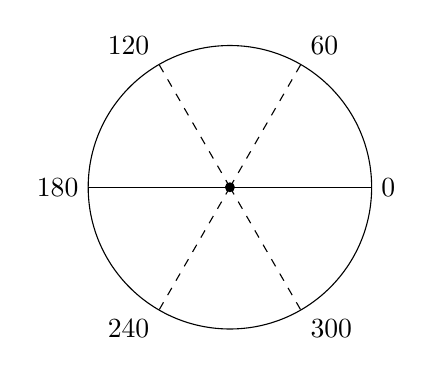
\begin{tikzpicture}[scale=1.8]
\coordinate (origin) at (0,0);
% Draw circle
\draw (origin) circle [radius=1];
% Draw axes
\draw (-1,0) node [left] {$180$} -- (1,0) node [right] {$0$};
% Draw other angles
\draw[dashed] (origin) -- +(60:1) node[above right] {$60$};
\draw[dashed] (origin) -- +(120:1) node[above left] {$120$};
\draw[dashed] (origin) -- +(240:1) node[below left] {$240$};
\draw[dashed] (origin) -- +(300:1) node[below right] {$300$};
% Dot at origin
\fill (origin) circle [radius=1pt];
\end{tikzpicture}
\hspace{5em}
% The unit circle divided into 30 degree segments
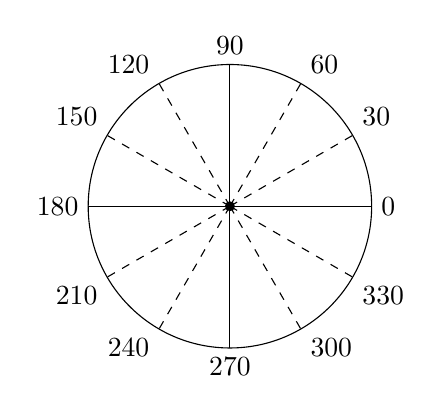
\begin{tikzpicture}[scale=1.8,baseline=-60pt]
\coordinate (origin) at (0,0);
% Draw circle
\draw (origin) circle [radius=1];
% Draw axes
\draw (-1,0) node [left] {$180$} -- (1,0) node [right] {$0$};
\draw (0,-1) node [below] {$270$} -- (0,1) node [above] {$90$};
% Draw other angles
\draw[dashed] (origin) -- +(30:1) node[above right] {$30$};
\draw[dashed] (origin) -- +(60:1) node[above right] {$60$};
\draw[dashed] (origin) -- +(120:1) node[above left] {$120$};
\draw[dashed] (origin) -- +(150:1) node[above left] {$150$};
\draw[dashed] (origin) -- +(210:1) node[below left] {$210$};
\draw[dashed] (origin) -- +(240:1) node[below left] {$240$};
\draw[dashed] (origin) -- +(300:1) node[below right] {$300$};
\draw[dashed] (origin) -- +(330:1) node[below right] {$330$};
% Dot at origin
\fill (origin) circle [radius=1pt];
\end{tikzpicture}
\end{center}

ברדיאנים:
\begin{center}
\selectlanguage{english}
% The unit circle with radians divided into pi/3 segments
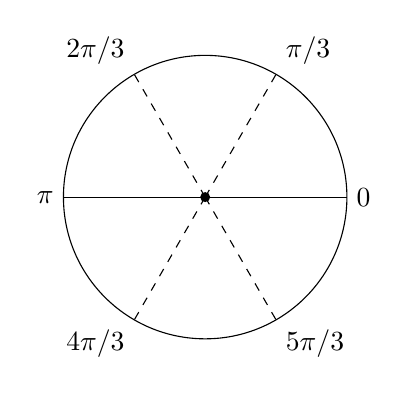
\begin{tikzpicture}[scale=1.8]
\coordinate (origin) at (0,0);
% Draw circle
\draw (origin) circle [radius=1];
% Draw axes
\draw (-1,0) node [left] {$\pi$} -- (1,0) node [right] {$0$};
% Draw other angles
\draw[dashed] (origin) -- +(60:1) node[above right] {$\pi/3$};
\draw[dashed] (origin) -- +(120:1) node[above left] {$2\pi/3$};
\draw[dashed] (origin) -- +(240:1) node[below left] {$4\pi/3$};
\draw[dashed] (origin) -- +(300:1) node[below right] {$5\pi/3$};
% Dot at origin
\fill (origin) circle [radius=1pt];
\end{tikzpicture}
\hspace{4em}
% The unit circle with radians divided into pi/6 segments
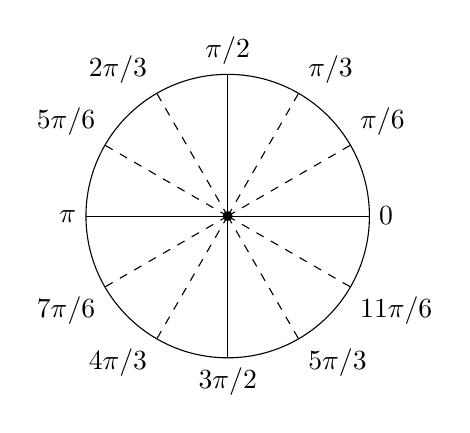
\begin{tikzpicture}[scale=1.8,baseline=-62pt]
\coordinate (origin) at (0,0);
% Draw circle
\draw (origin) circle [radius=1];
% Draw axes
\draw (-1,0) node [left] {$\pi$} -- (1,0) node [right] {$0$};
\draw (0,-1) node [below] {$3\pi/2$} -- (0,1) node [above] {$\pi/2$};
% Draw other angles
\draw[dashed] (origin) -- +(30:1) node[above right] {$\pi/6$};
\draw[dashed] (origin) -- +(60:1) node[above right] {$\pi/3$};
\draw[dashed] (origin) -- +(120:1) node[above left] {$2\pi/3$};
\draw[dashed] (origin) -- +(150:1) node[above left] {$5\pi/6$};
\draw[dashed] (origin) -- +(210:1) node[below left] {$7\pi/6$};
\draw[dashed] (origin) -- +(240:1) node[below left] {$4\pi/3$};
\draw[dashed] (origin) -- +(300:1) node[below right] {$5\pi/3$};
\draw[dashed] (origin) -- +(330:1) node[below right] {$11\pi/6$};
% Dot at origin
\fill (origin) circle [radius=1pt];
\end{tikzpicture}
\end{center}

\np

נחשב את הסינוס של 
$\angle BAC = 30^\circ$.
במשולש ישר-זווית
$\triangle ACB$
עם יתר באורך 
$1$:
\begin{center}
\selectlanguage{english}
% Right triangle with 30 and 60 degree angles
\begin{tikzpicture}[scale=6]
% Coordinates
\coordinate (origin) at (0,0);
\coordinate (lower-right) at (1,0);
\coordinate (upper-right) at (1,.5);
% Draw triangle
\draw (origin)
  node[left] {$A$} node[above right,xshift=24pt] {$30$} --
  node[below] {$b=\cos 30$} (lower-right) node[right] {$C$} --
  node[right] {$a=\sin 30$} (upper-right)
  node[right] {$B$} node[below left,yshift=-5pt] {$60$} --
  cycle;
% Get intersection of hypotenuse with line at 30 degrees
\path[name path=hypotenuse] (origin) -- (upper-right);
\path[name path=to-hyp] (lower-right) -- +(150:6mm);
\path[name intersections={of=hypotenuse and to-hyp,by=on-hyp}];
% Draw the line and label the angles
\draw (lower-right) 
    node[above left,yshift=5pt,xshift=2pt] {$60$}
    node [left,yshift=6pt,xshift=-16pt] {$30$} --
    (on-hyp)
    node[right,xshift=8pt] {$60$}
    node[below,yshift=-4pt] {$120$}
    node[above] {$D$};
% Label line segments
\path (lower-right) -- node[above] {$a$} (on-hyp);
\path (on-hyp) -- node[above] {$a$} (upper-right);
\path (origin) -- node[above,yshift=4pt] {$1-a$} (on-hyp);
% Square for right angle
\draw (lower-right) rectangle +(-1pt,1pt);
\end{tikzpicture}
\end{center}

צייר קו
$CD$
אל היתר כך ש-%
$\angle DCA=30^\circ$.
כדי להשלים ל-%
$180^\circ$
במשלוש,
$\angle ADC=120^\circ$,
וניתן לחשב את שאר הזוויות.
$\triangle BCD$
שווי-צלעות ולכן
$DC=a=\sin 30^\circ$.
$\triangle ACD$
שווי-שוקיים כך ש-%
$a=1-a$
ו-%
$\sin 30^\circ = a = \frac{1}{2}$.
ערך הקוסינוס הוא:
\[
\cos 30^\circ = \sqrt{1-\sin^2 30^\circ} = \sqrt{1-\left(\frac{1}{2}\right)^2} = \sqrt{\frac{3}{4}} = \frac{\sqrt{3}}{2}\,.
\]

%%%%%%%%%%%%%%%%%%%%%%%%%%%%%%%%%%%%%%%%%%%%%%%%%%%%%%%%%%%%%%%

\vspace{-4ex}

\section*{סינוס וקוסינוס של
$(90\!-\!\theta)$}
הצלע הנגדי לזווית מתחלף עם הצלע השכן של הזוויות ומכאן:
\[
\cos (90\!-\!\theta) = \sin \theta,\quad\quad \sin (90\!-\!\theta) = \cos \theta\,.
\]

\vspace{-2ex}

\begin{center}
\selectlanguage{english}
% Quadrant with angles 90 and 90 - theta
\begin{tikzpicture}[scale=2.5]
\coordinate (origin) at (0,0);
% Draw arc
\draw[name path=arc] (1,0) arc [start angle=0, end angle=90, radius=1];
% Draw x-axis
\draw[name path=x] (origin) -- (1,0);
% Draw y-axis
\draw (origin) -- (0,1);
% Draw ray
\draw[rotate=30,name path=ray] (origin) node [above right,xshift=8mm] {$\theta$} -- node [above] {$1$} (1,0);
% Get intersection of arc and ray
\path [name intersections={of=ray and arc, by=on-circle}];
% Draw altitude from intersection to x-axis
\draw[name path=altitude] (on-circle) node [above right] {$90-\theta$} -- node [right,xshift=4mm] {$\sin \theta = \cos (90\!-\!\theta)$} (on-circle |- origin);
% Arrow from label
\draw[->] (1,.5) -- +(-.2,-.1);
% Get intersection of altitude and x-axis
\path [name intersections={of=altitude and x, by=on-x}] (origin) -- node [below] {$\cos \theta = \sin (90\!-\!\theta)$} (on-x);
% Square for right angle at intersection
\draw (on-x) rectangle +(-1pt,1pt);
\fill (origin) circle [radius=.5pt];
\end{tikzpicture}
\end{center}

\vspace{-3ex}

\section*{%
סינוס וקוסינוס של
$2\theta$%
}

את הנוסחאות ל-%
$\sin 2\theta,\cos 2\theta$
ניתן לשחזר מהנוסחאות לחיבור של זוויות הניתנות בנוסחאון:
\erh{0pt}
\begin{equationarray*}{rcl}
\sin 2\theta &=& \sin (\theta+\theta)\\
&=&\sin \theta \cos \theta + \sin \theta \cos \theta\\
&=& 2\sin \theta \cos \theta\\
\cos 2\theta &=& \cos (\theta+\theta)\\
&=&\cos \theta \cos \theta - \sin \theta \sin \theta\\
& =& \cos^2 \theta - \sin^2 \theta\\
&=&(1-\sin^2 \theta) - \sin^2 \theta\\
&=& 1 - 2\sin^2 \theta\,.
\end{equationarray*}

\npchap
